\Tsubsection{UI1 Sitio} 

\Large{\textbf{Objetivo}}\\\\
\normalsize{Texto}\\

	

\Large{\textbf{Descripción}}\\
\normalsize{Texto}\\

\Large{\textbf{Comandos}}\\
\normalsize{}

\begin{itemize}
	\item Lorem ipsum
	\item Lorem ipsum
	\item Lorem ipsum
\end{itemize}


\Large{\textbf{Referencia}}\\\\
\normalsize{\Tref{CU1}{CU1 Mostrar noticias},\Tref{CU7}{CU7 Ingresar a sitio web}}

\begin{figure}[H]\Tlabel{UI1}
  \centering
	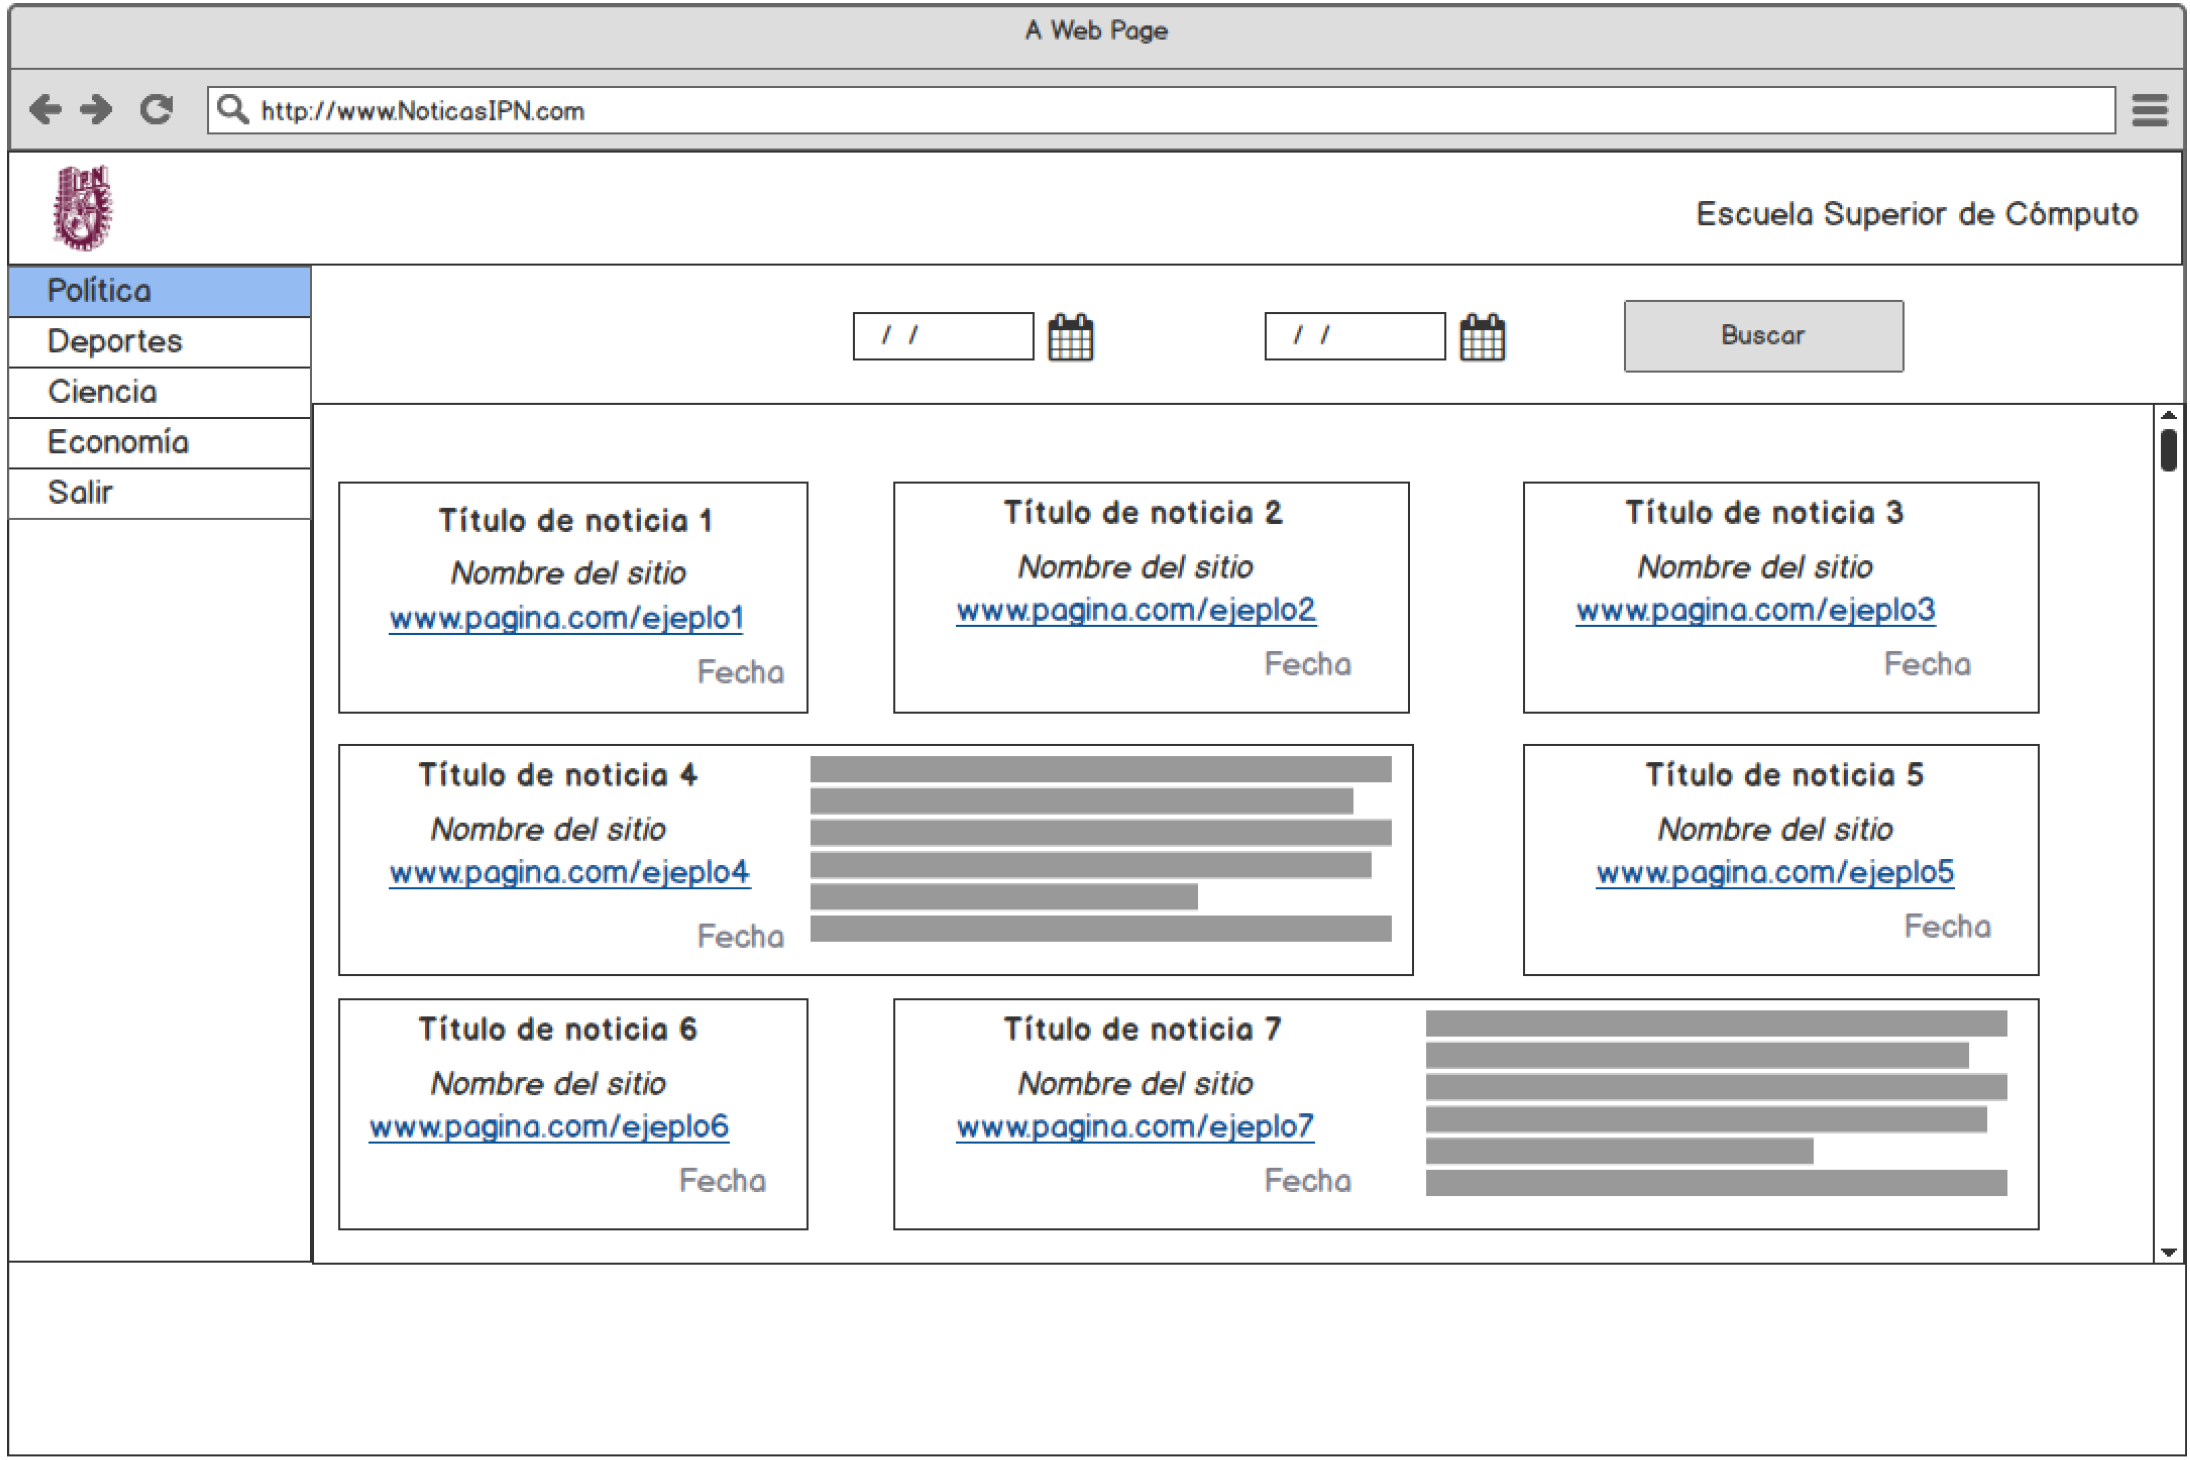
\includegraphics[scale=.35]{imagenes/Pantallas/UI1}
  \caption{Pantalla UI1 Inico}
  \label{fig:UI1}
\end{figure}



\begin{figure}[H]\Tlabel{UI2}
  \centering 
	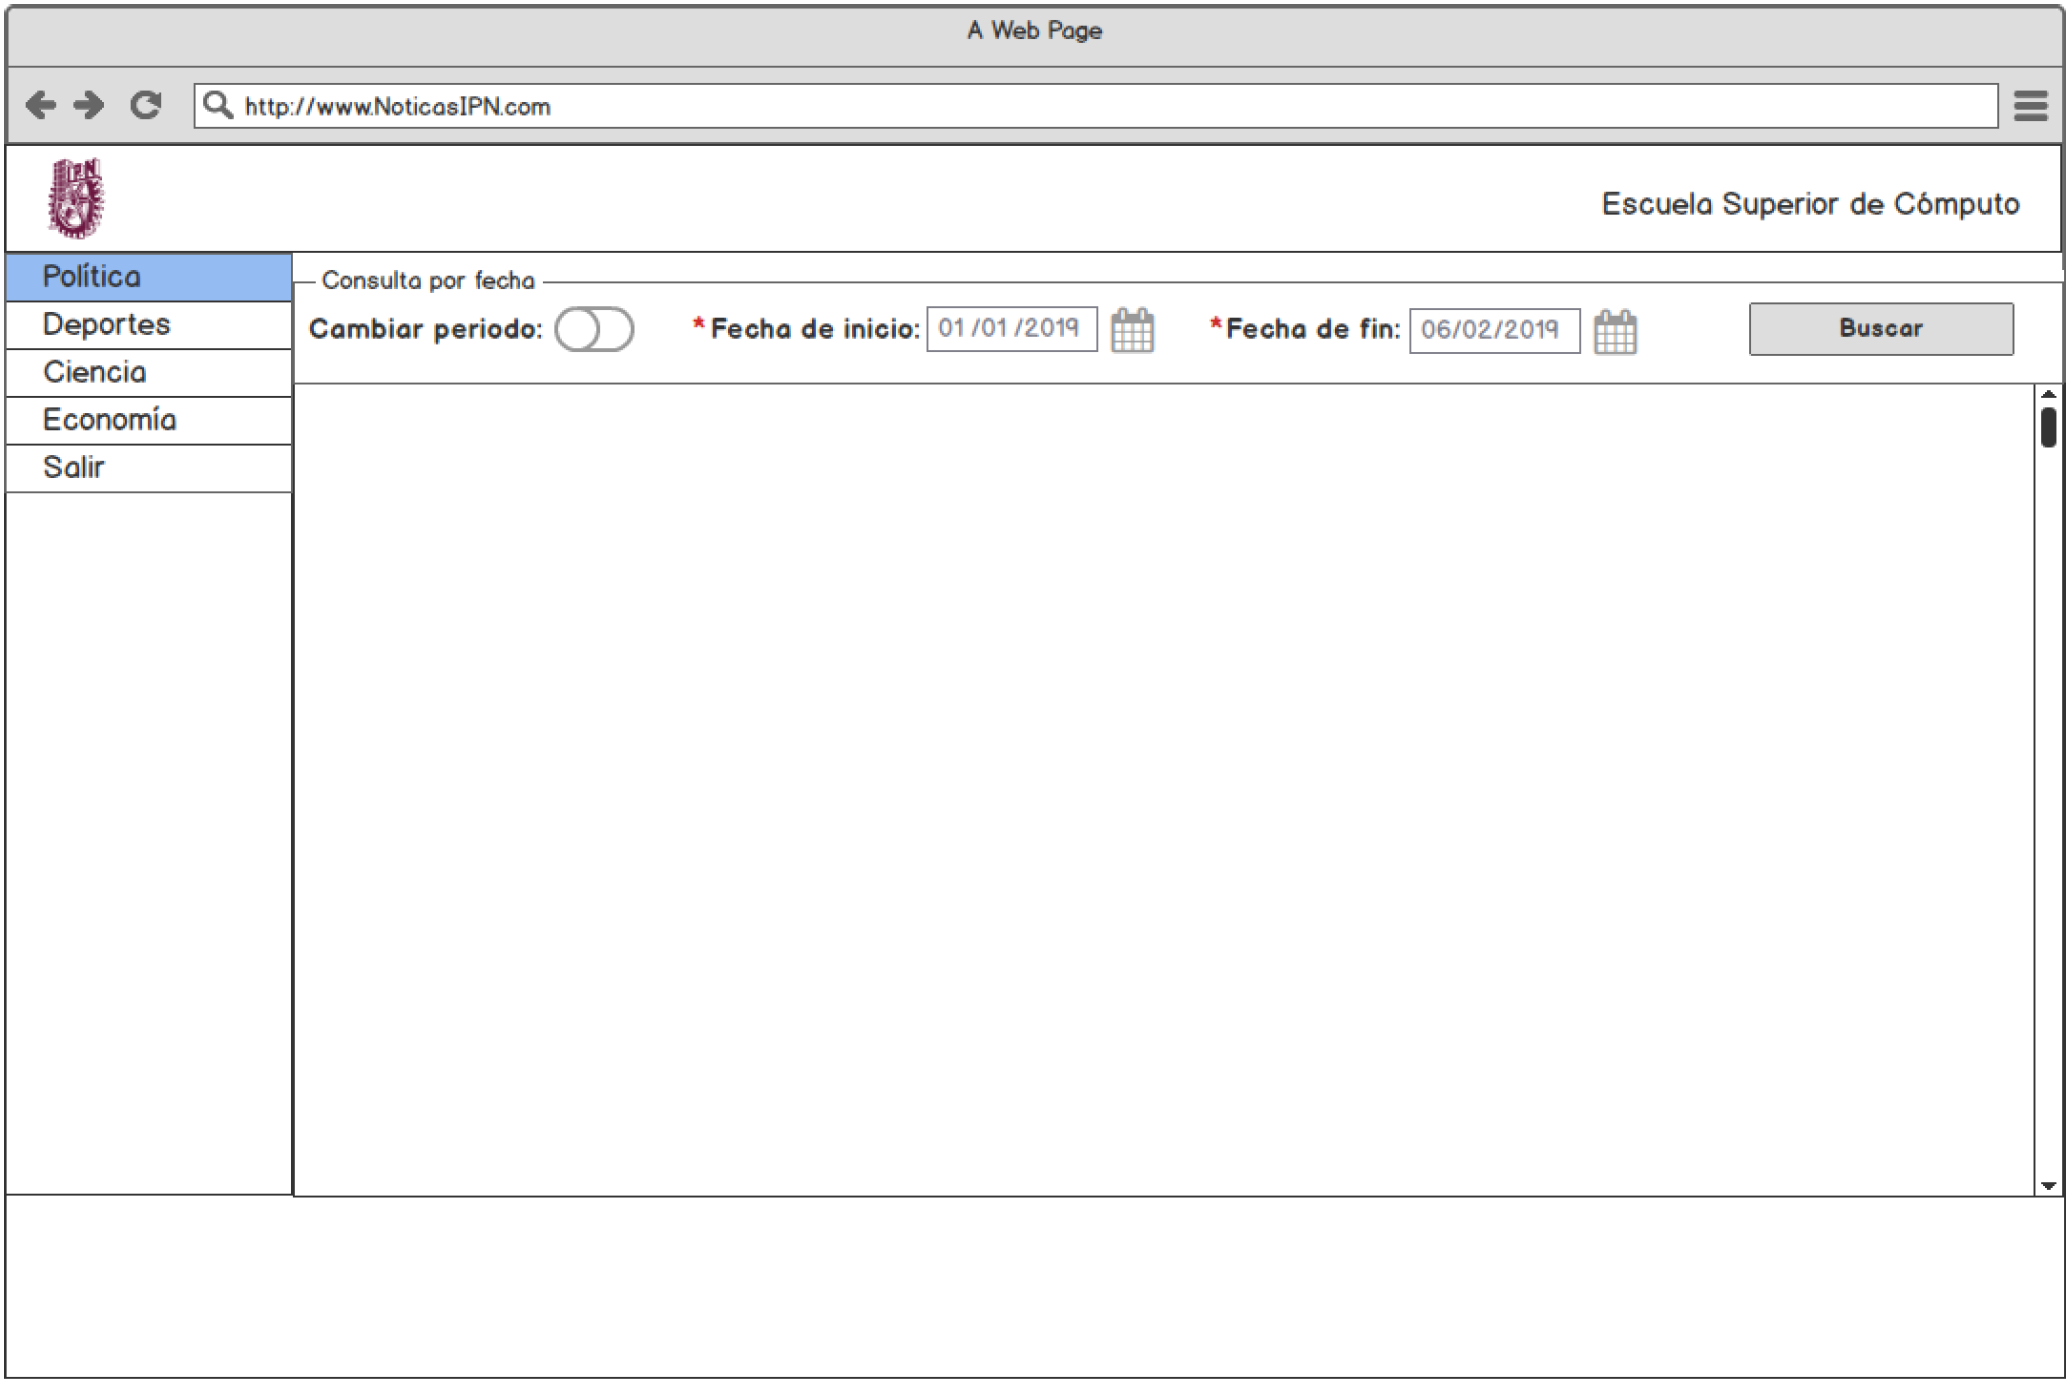
\includegraphics[scale=.35]{imagenes/Pantallas/UI2}
  \caption{Pantalla UI2 Sección política}
  \label{fig:UI2}
\end{figure}



\begin{figure}[H]\Tlabel{UI3}
  \centering
	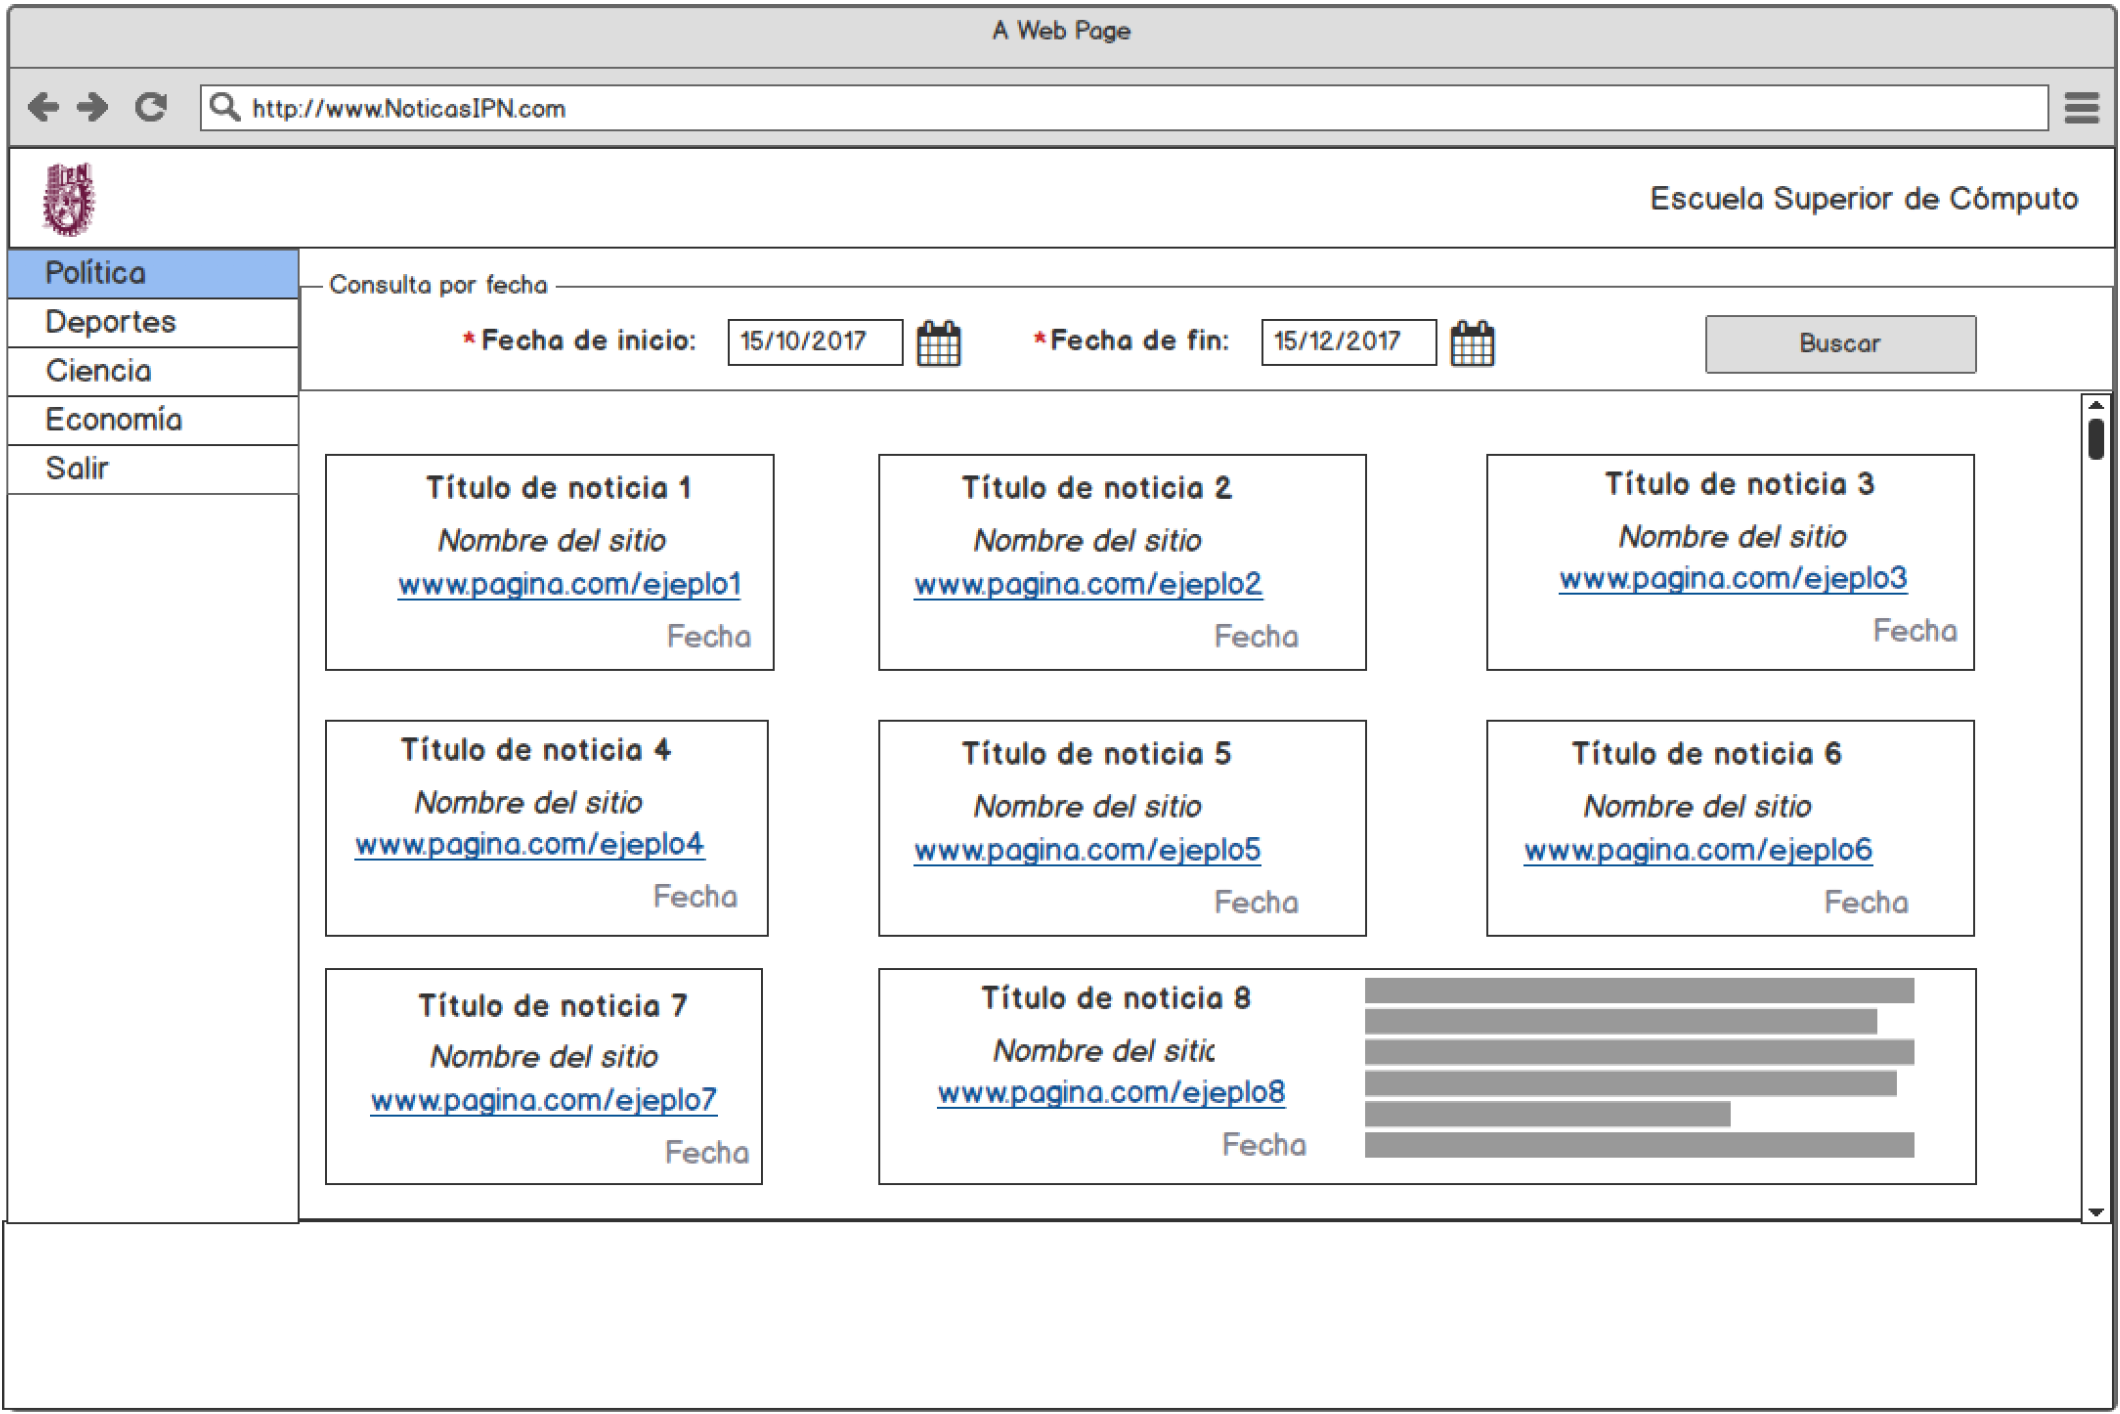
\includegraphics[scale=.35]{imagenes/Pantallas/UI3}
  \caption{Pantalla UI3 Cambio de periodo}
  \label{fig:UI3}
\end{figure}


\begin{figure}[H]\Tlabel{UI4}
  \centering
	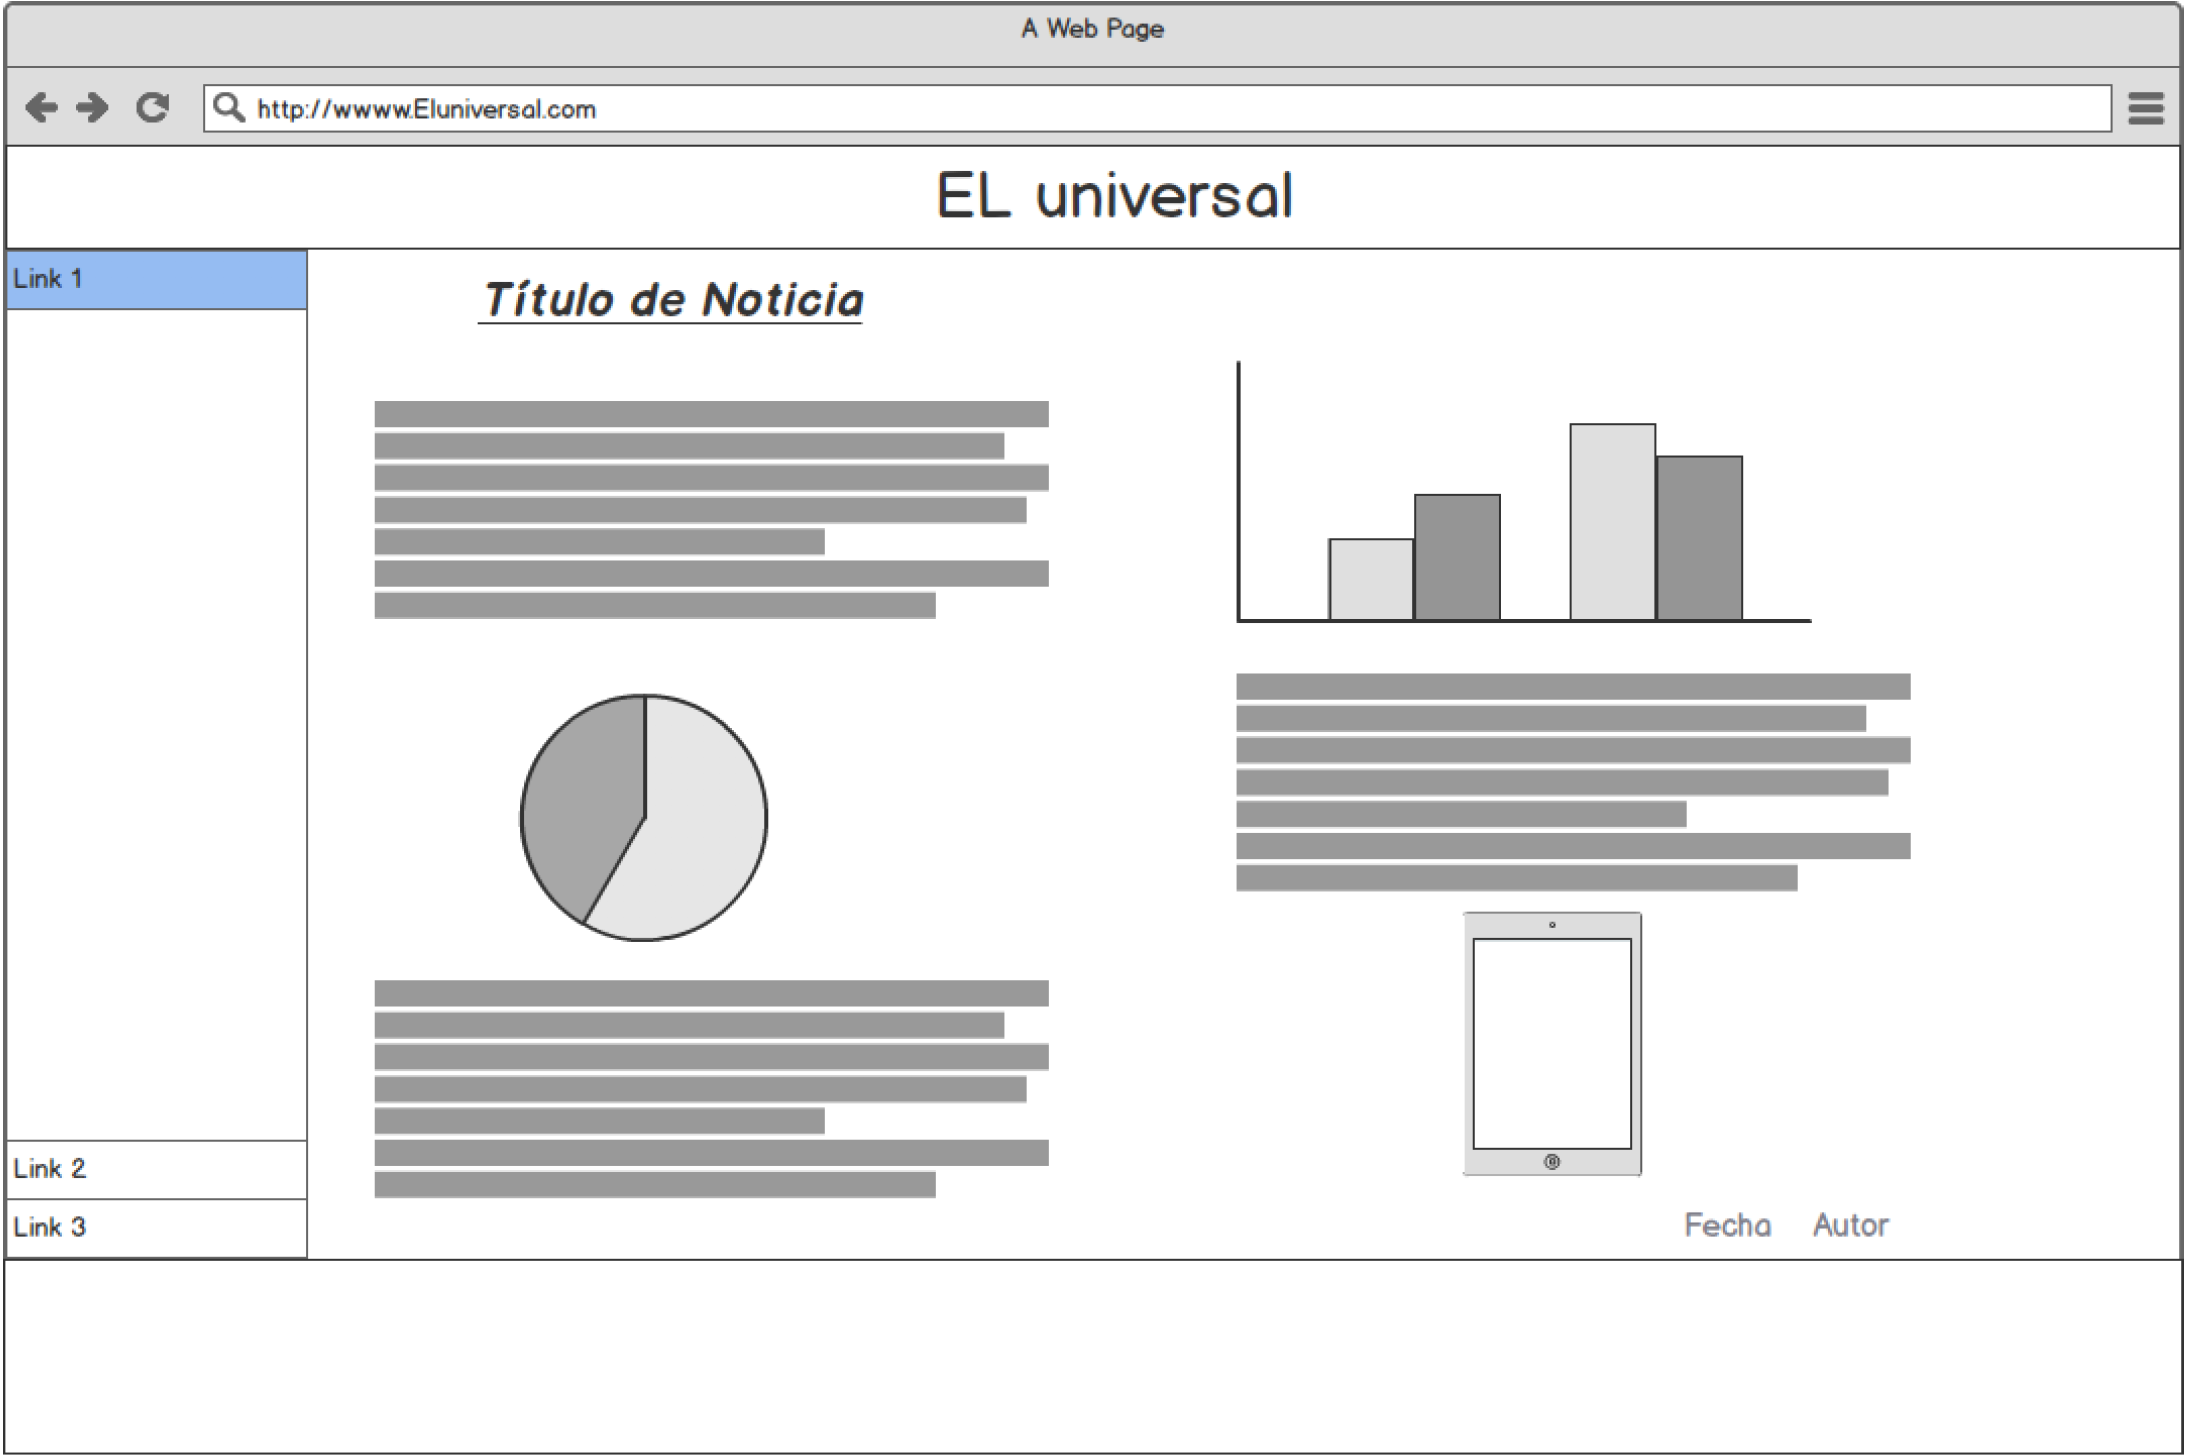
\includegraphics[scale=.35]{imagenes/Pantallas/UI4}
  \caption{Pantalla UI4 Página de sitio web}
  \label{fig:UI4}
\end{figure}